\section{How to use WS-Attacker}
\label{sec:how_to_use_ws_attacker}

This guide will use WS-Attacker for penetration testing on self-made web service.
In general, you have to to four things:

\begin{enumerate}
    \item Loading the WSDL and set up the request parameters.
    \item Submitting a test request.
    \item Configuring the attack plugins.
    \item Starting the attacks.
\end{enumerate}

\subsection{Loading a WSDL}
\label{sec:loading_a_wsdl}

After starting WS-Attacker, the GUI appears and offers an input field to enter the location
of the WSDL, see Figure \ref{fig:load_wsdl}.

\begin{figure}[h!]
    \begin{center}
        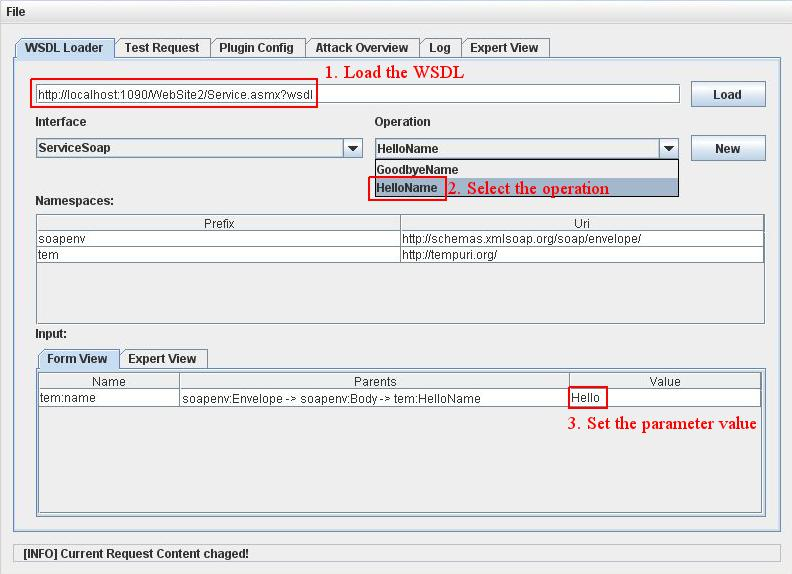
\includegraphics[width=0.8\textwidth]{img/load_wsdl}
    \end{center}
    \caption{Loading the WSDL.}
    \label{fig:load_wsdl}
\end{figure}

The custom service has two operations: \emph{HelloName} and \emph{GoodbyeName}.
\emph{HelloName} is chosen as the operation to be tested. The table at the bottom gives a
form based input possibility for all request parameters and in this case, \emph{name} is set to
\emph{Hello}.

\subsection{Submitting a Test Request}
\label{sec:submitting_a_test_request}

Next step is to do a test request: Figure \ref{fig:test_request} shows
the test request and the corresponding response. The request contains a
\enquote{HelloName} element as first body child and the response holds the
corresponding element \enquote{HelloNameResult}. This request is very important
as attack plugins will use its response for comparing it with the responses of
the attack request. This allows to check, what has really changed due to attack
modifications. 

\begin{figure}[h!]
    \begin{center}
        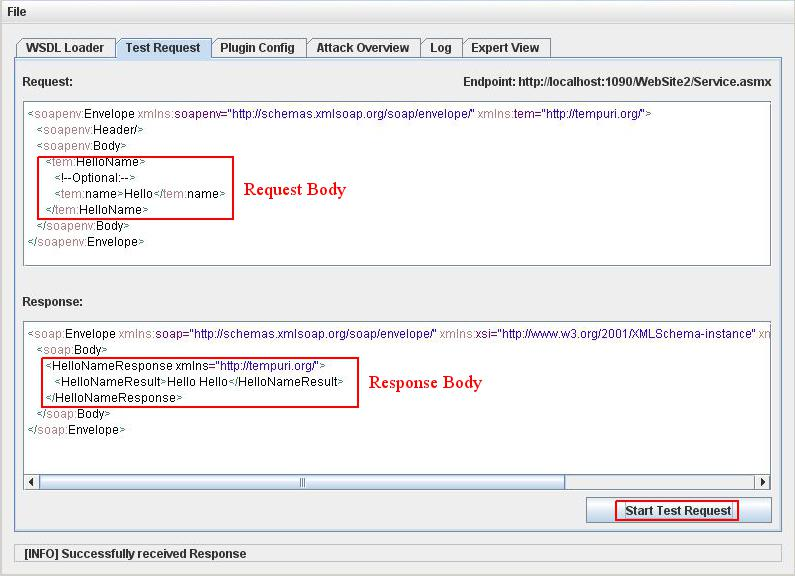
\includegraphics[width=0.8\textwidth]{img/test_request}
    \end{center}
    \caption{Submitting a test request.}
    \label{fig:test_request}
\end{figure}

\subsection{Attack Plugin Configuration}
\label{sec:attack_plugin_configuration}

The next step is to configure the plugins. In this case, the automatic mode is
used for SOAPAction Spoofing (Figure \ref{fig:plugin_config_sas}) and
the WS-Addressing Spoofing plugin detects the endpoint URL automatically
(Figure \ref{fig:plugin_config_wsas}), too -- there is nothing to
configure manually. The tree on the left shares different views on the plugins.
\emph{Active Plugins} contains all plugins which will be used for attacking the
server, \emph{All Plugins} contains all plugins ordered by their category and
\emph{Alphabetical Sorted} shows all plugins in an alphabetical order.

\begin{figure}[h!]
    \begin{center}
        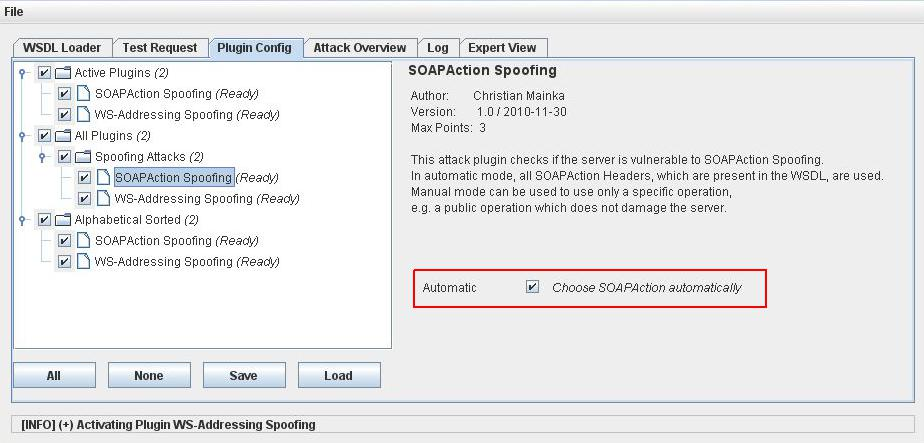
\includegraphics[width=0.8\textwidth]{img/plugin_config_sas}
    \end{center}
    \caption{Plugin configuration for SOAPAction Spoofing.}
    \label{fig:plugin_config_sas}
\end{figure}

\begin{figure}[h!]
    \begin{center}
        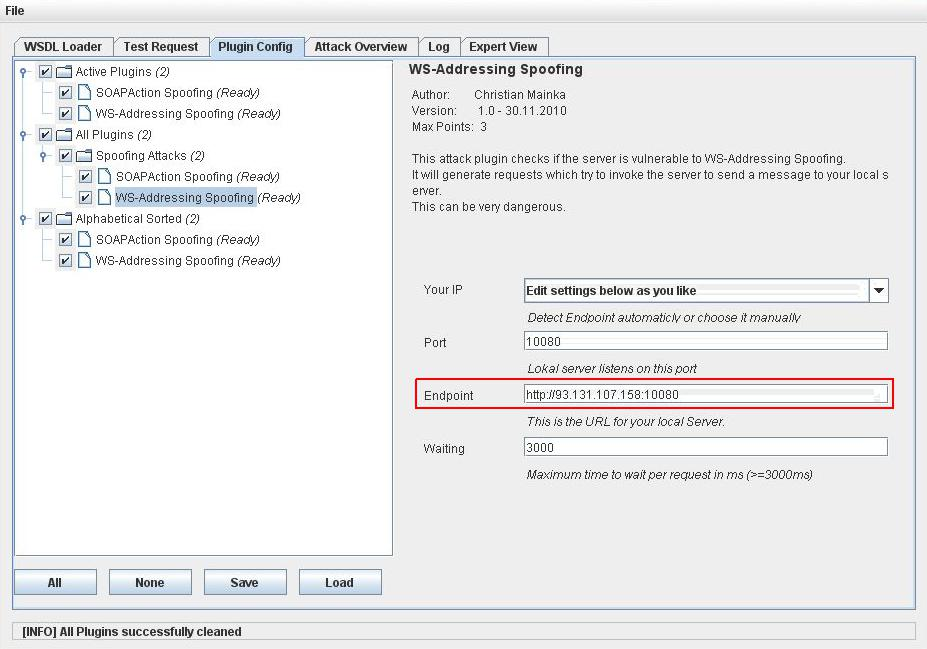
\includegraphics[width=0.8\textwidth]{img/plugin_config_wsas}
    \end{center}
    \caption{Plugin configuration for WS-Addressing Spoofing.}
    \label{fig:plugin_config_wsas}
\end{figure}

\subsection{Starting the Attacks}
\label{sec:starting_the_attacks}

The last step is to start the attack. Figure \ref{fig:attack_done} shows
the overview of a finished attack run. Active plugins are displayed on the top,
their results at the bottom. The slider in the top part allows to filter the
results by their level. The user can choose to see only the most
\emph{important} results, or see even the request content at the \emph{tracing}
level.

\begin{figure}[h!]
    \begin{center}
        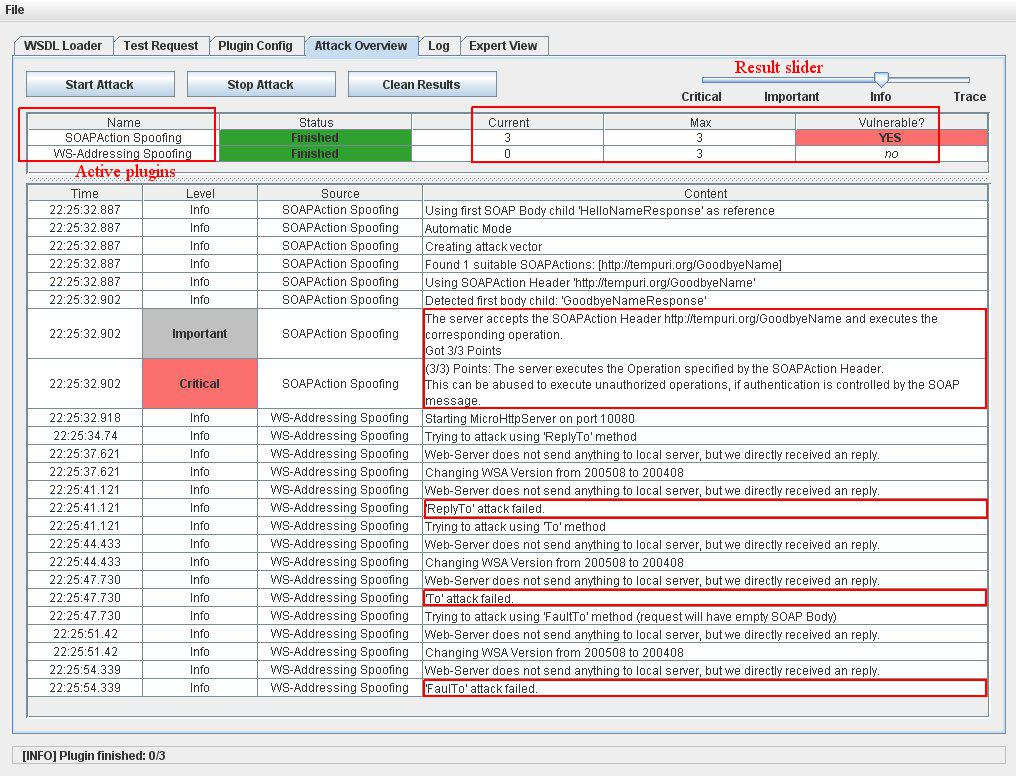
\includegraphics[width=0.8\textwidth]{img/attack_done}
    \end{center}
    \caption{Penetration test on .NET finished.}
    \label{fig:attack_done}
\end{figure}

The web service is vulnerable to SOAPAction Spoofing but resistant to
WS-Addressing Spoofing. This is indicated different aspects:

\begin{enumerate}
    \item The \emph{vulnerable} column values show \textbf{YES} for SOAPAction Spoofing and \emph{no} for WS-Addressing Spoofing.
    \item The SOAPAction Spoofing plugin got the maximum rating -- three of three points in this case -- and WS-Addressing Spoofing got zero points.
    \item The results show, that the server has executed the operation defined
        in the SOAPAction Header, which is the most critical security issue.
\end{enumerate}
